
\newcommand{\audioparameter}[4]{\vspace{3mm}
\begin{tcolorbox}[colback=parambackground,
	colframe=white!20!black,
	center,
	valign=top,
	halign=left,
	center title,
	width=\textwidth]

	\begin{tabular}{p{0.06\textwidth}p{0.4\textwidth}p{0.2\textwidth}p{0.2\textwidth}}
		\raisebox{-.32\height}{
\includegraphics[width=0.06\textwidth]{graphics/knob.png}} & \underline{\fat{\large{#1}}}&  \small{Modulatable}:
		\IfEqCase{#2}{%
        	{1}{
\includegraphics[width=0.025\textwidth]{graphics/available.png}}%
        	{0}{
\includegraphics[width=0.02\textwidth]{graphics/not_available.png}}%
		}[\PackageError{audioparameter}{Undefined option to param: #2}{}] 
		&\small{Automatable}:
		\IfEqCase{#3}{%
		{1}{
\includegraphics[width=0.025\textwidth]{graphics/available.png}}%
		{0}{
\includegraphics[width=0.02\textwidth]{graphics/not_available.png}}%
		}[\PackageError{audioparameter}{Undefined option to param: #3}{}] 
		\\
	\end{tabular}

	\vspace{5mm}
	#4
\end{tcolorbox}
}
\newcommand{\audioparameterint}[1]{\vspace{3mm}\noindent\textbf{Parameter: #1} [modulatable, whole numbers]\\}
\newcommand{\modmatrix}{\hyperref[chapter_matrix]{modulation matrix}\hspace{1mm}}
\newcommand{\fat}{\textbf}


% \newcommand{\tree}[2]{%
%     \IfEqCase{#1}{%
%         {a}{$\sqrt{#2}$}%
%         {b}{Hi}%
%         % you can add more cases here as desired
%     }[\PackageError{tree}{Undefined option to tree: #1}{}]%
% }%

\documentclass[12pt]{report}
\usepackage{graphicx}
\usepackage{hyperref}
\usepackage{svg}
\usepackage{mwe}
\usepackage{xcolor}
\usepackage[many]{tcolorbox}
\usepackage[margin=1in]{geometry}
\usepackage{xstring}
\usepackage{utopia}
\usepackage{pagecolor}
\usepackage{array}
\usepackage{longtable}
\usepackage{titlesec} 
\usepackage{lipsum} % just to generate text for the example

\titleformat{\chapter}[display]
  {\bfseries\Huge}
  {}%\filright\MakeUppercase{\chaptertitlename} \Huge\thechapter}
  {1ex}
  {\titlerule\vspace{1ex} \chaptertitlename \hspace{3mm} \Huge\thechapter \hfill}
  [\vspace{1ex}\titlerule]



\newcolumntype{L}[1]{>{\raggedright\let\newline\\\arraybackslash\hspace{0pt}}m{#1}}


\definecolor{parambackground}{rgb}{0.9470, 0.963, 1}

%\titleformat{\chapter}[hang]{\Huge\bfseries}{\thechapter\hsp\textcolor{gray75}{|}\hsp}{0pt}{\Huge\bfseries}
\begin{document}
\pagecolor{white!95!black}
\setlength{\parindent}{0pt}
\begin{titlepage}
	\mbox{}
	\centering
	\vspace{20mm}
	
	{\Huge\bfseries Odin 2\par}
	{\huge\bfseries Synthesizer Plugin\par}
	\vspace{2cm}
	{\Huge\bfseries Manual\par}
	{\Large\bfseries for version 2.2.0\par}
	\vspace{2cm}
	{\Large TheWaveWarden\par}
	
\includegraphics[width=0.4\textwidth]{graphics/logo.png}\par
	{\large \url{www.thewavewarden.com}\par}

	\vspace{10mm}

	\begin{center}
		\begin{tabular}{p{0.2\textwidth}p{0.15\textwidth}p{0.2\textwidth}p{0.15\textwidth}p{0.25\textwidth}}
			&
\includegraphics[width=0.15\textwidth]{graphics/vst3_logo.png}& & 
\includegraphics[width=0.11\textwidth]{graphics/au_logo.png}&
		\end{tabular}
	\end{center}

	\vfill

	% Bottom of the page
	{\large \today\par}
\end{titlepage}
\clearpage

\tableofcontents
\clearpage

\chapter{Introduction}

%This manual aims to get new users started with the Odin 2 synthesizer plugin and provide a detailed documentation for experienced users.

\section{Install}
You can download Odin 2 from \url{https://www.thewavewarden.com/odin2}. Make sure to download the correct installer for your platform.

\vspace{3mm}
\fat{Windows}:

The install wizard will guide you through the process on Windows systems.

\vspace{3mm}
\fat{MacOS}:

The install wizard gives you the option to install either the VST3 or AudioUnit plugins. Installing the AudioUnit version is only recommended for users of Apples Digital Audio Workstation "Logic".

\vspace{3mm}
\fat{GNU/Linux}

For GNU/Linux based systems you have two options: Debian based operating systems (Debian, Ubuntu, Mint and many more) can use the convenient Debian packages (.deb file) to install Odin. Other distributions have to use the manual installer. Open the README.txt file in the zip for further installation instructions in that case.
All installers will install the VST3 version, as well as the LV2 version of Odin2.

\vspace{5mm}
\begin{tcolorbox}[colback=yellow!10!white,
    colframe=white!20!black,
    center,
    valign=top,
    halign=left,
    center title,
    width=\textwidth]

    Please note that \fat{Odin 2 is not available as a 32Bit plugin} due to build complications.
    
    Furthermore,\fat{ Odin 2 is not available as a VST2 plugin} due to the ended licensing on behalf of Steinberg Media Technologies.
\end{tcolorbox}

\vspace{5mm}
\fat{Adding Odin 2 to a Track}

\vspace{5mm}
Odin 2 can be added to your track like any other VST3, AudioUnit or LV2 plugin. For details on how to add the plugin in your Digital Audio Workstation, refer to its manual.

\clearpage
\section{Odin 2: A Mighty God}
\begin{center}
    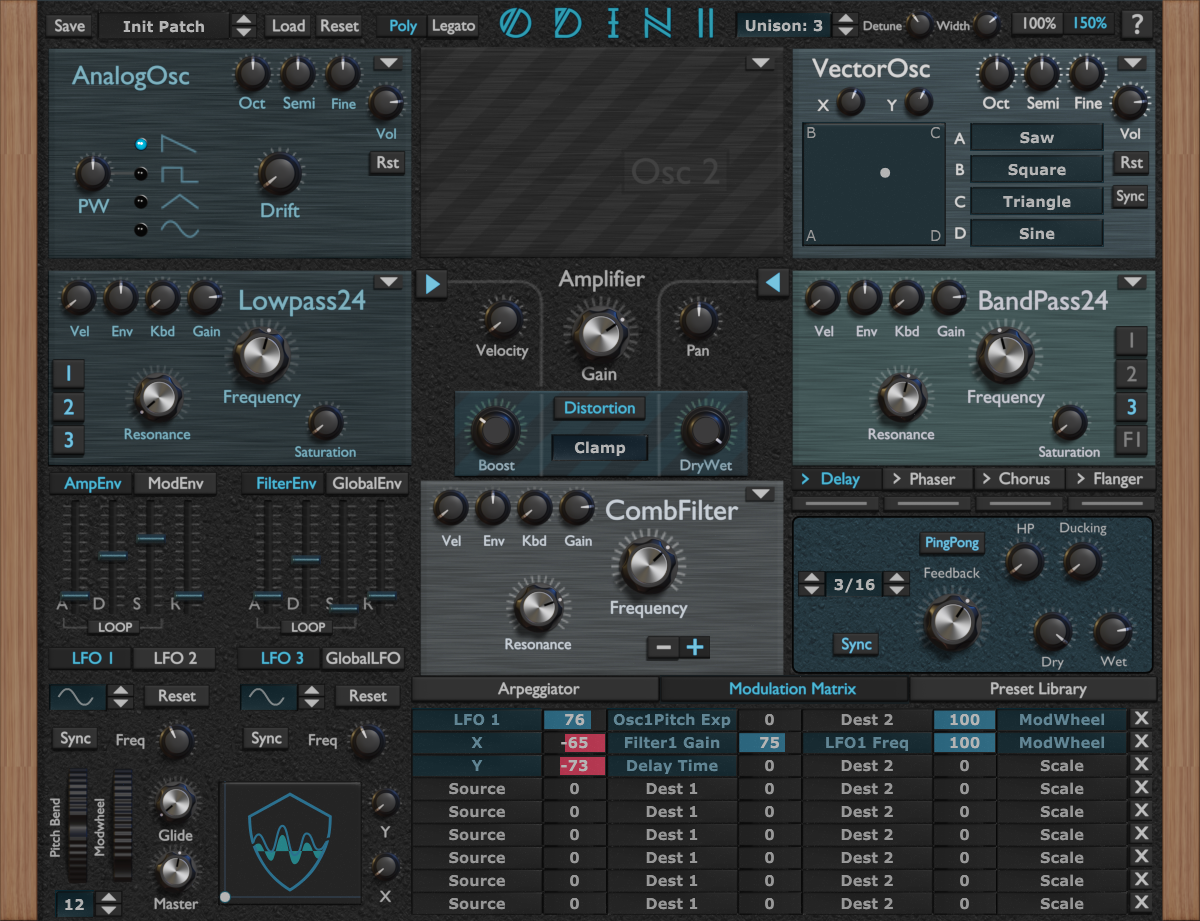
\includegraphics[width=\textwidth]{graphics/mighty_god.png}
\end{center}

Odin 2 is a mighty kick-ass semimodular subtractive synthesizer plugin, which is \fat{made for you with love}. Oh, also, it is

\begin{center}
    \fat{\large{Free Software!}}.
\end{center}

Don't let anybody tell you otherwise. 

\vspace{1mm}
The design approach of Odin 2 lets you choose from a large variety of modules, which can be mixed and matched for virtually endless sonic capabilities. Three Oscillators, three Filters, a dedicated Distortion, four onboard FX, four Envelopes, four LFOs ... the list continues: Modulate tons of parameters with the big-ass Modulation Matrix, use the Arpeggiator and Step Sequencer to generate rhythms and musical ideas, there's Unison, a XY-Pad, you can draw your oscillator waves, or maybe your spectra?

\vspace{2mm}
This text is supposed to fit on one page, so I can't really talk about everything Odin 2 has to offer,

\begin{center}
    \fat{\large{but}}
\end{center}

The sonic capabilities of Odin 2 will keep you happy for years to come, so dig right into it and get started!

\clearpage
\section{Panel Overview}
\begin{center}
    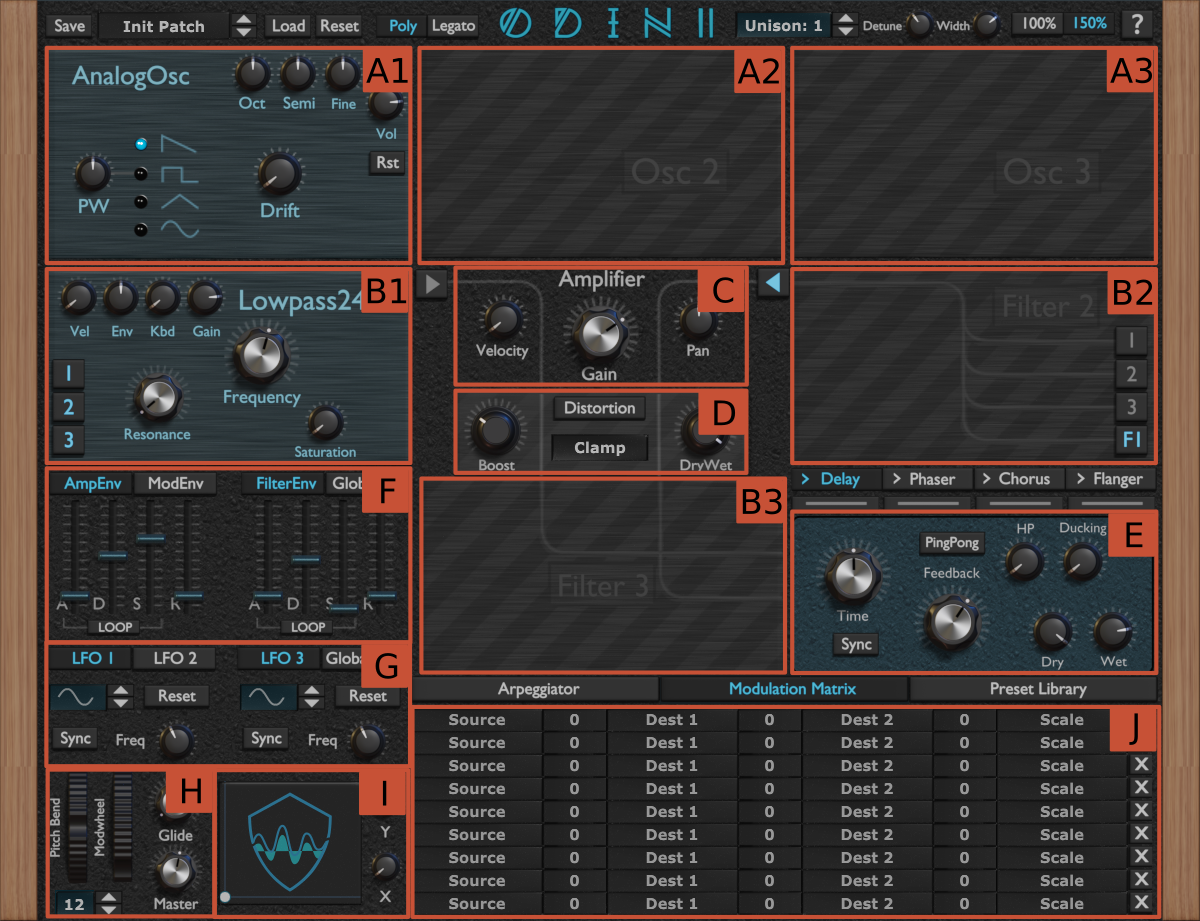
\includegraphics[width=\textwidth]{graphics/overview.png}
\end{center}

\begin{itemize}
    \item \fat{A}: The three oscillator slots. See Chapter \ref{oscillators}.
    \item \fat{B}: The three filter slots. See Chapter \ref{filters}.
    \item \fat{C}: The amplifier module. See Chapter \ref{amplifier}.
    \item \fat{D}: The distortion module. See Chapter \ref{distortion}.
    \item \fat{E}: The FX section: See Chapter \ref{FX}.
    \item \fat{F}: The four ADSR Envelopes. See Chapter \ref{ADSR}
    \item \fat{G}: The four Low Frequency Oscillators (LFOs). See Chapter \ref{LFOs}
    \item \fat{H}: The global controls See Chapter \ref{global}
    \item \fat{I}: The XY-pad section. See Section \ref{xy}
    \item \fat{J}: The \modmatrix. This space can also be occupied by the Arpeggiator (Chapter \ref{arpeggiator}) and Preset Browser (Section \ref{presets}).
\end{itemize}
\section{Saving and Loading Presets}
\label{presets}

So you just downloaded the synth and want to see what is it capable of or stumbled upon a cool sound which you want to save for later. Both of these are done in the \fat{Preset Library}:

\begin{center}
    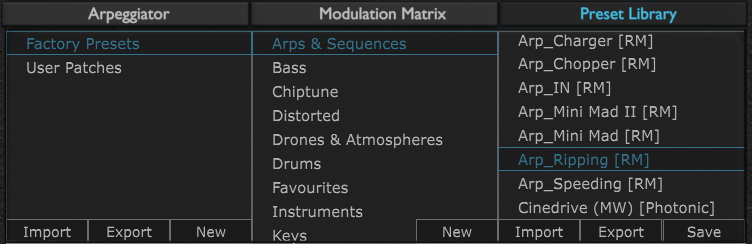
\includegraphics[width=\textwidth]{graphics/preset_browser.png}
\end{center}

\begin{tcolorbox}[colback=yellow!10!white,
    colframe=white!20!black,
    center,
    valign=top,
    halign=left,
    center title,
    width=\textwidth]

    The Preset Browser occupies the same space in the GUI as the Modulation Matrix and the Arpeggiator. If you can't locate the module in the lower right corner of the GUI, press the "Preset Library" button above the modulation matrix:

    \begin{center}
        
\includegraphics[width=\textwidth]{graphics/preset_browser_button.png}
    \end{center}
\end{tcolorbox}

The preset browser is divided into the "Soundbank Selection" (left), the "Category Selection" (mid) and the "Patch Selection" (right).

\vspace{5mm}
\fat{Loading Presets}:

To load a preset, navigate to the desired soundbank and category and click on a preset.

\vspace{5mm}
\fat{Saving Presets}:

To save a preset, navigate to the desired soundbank and category and click the "Save" button in the bottom right corner of the module. A text field will appear, where you can input a name for the preset. Pressing the enter-key or "Save" again will save the preset to the current category.

\clearpage
\section{Routing}
\label{routing}

Here's an overview of the internal signal flow inside Odin 2:
\begin{center}
    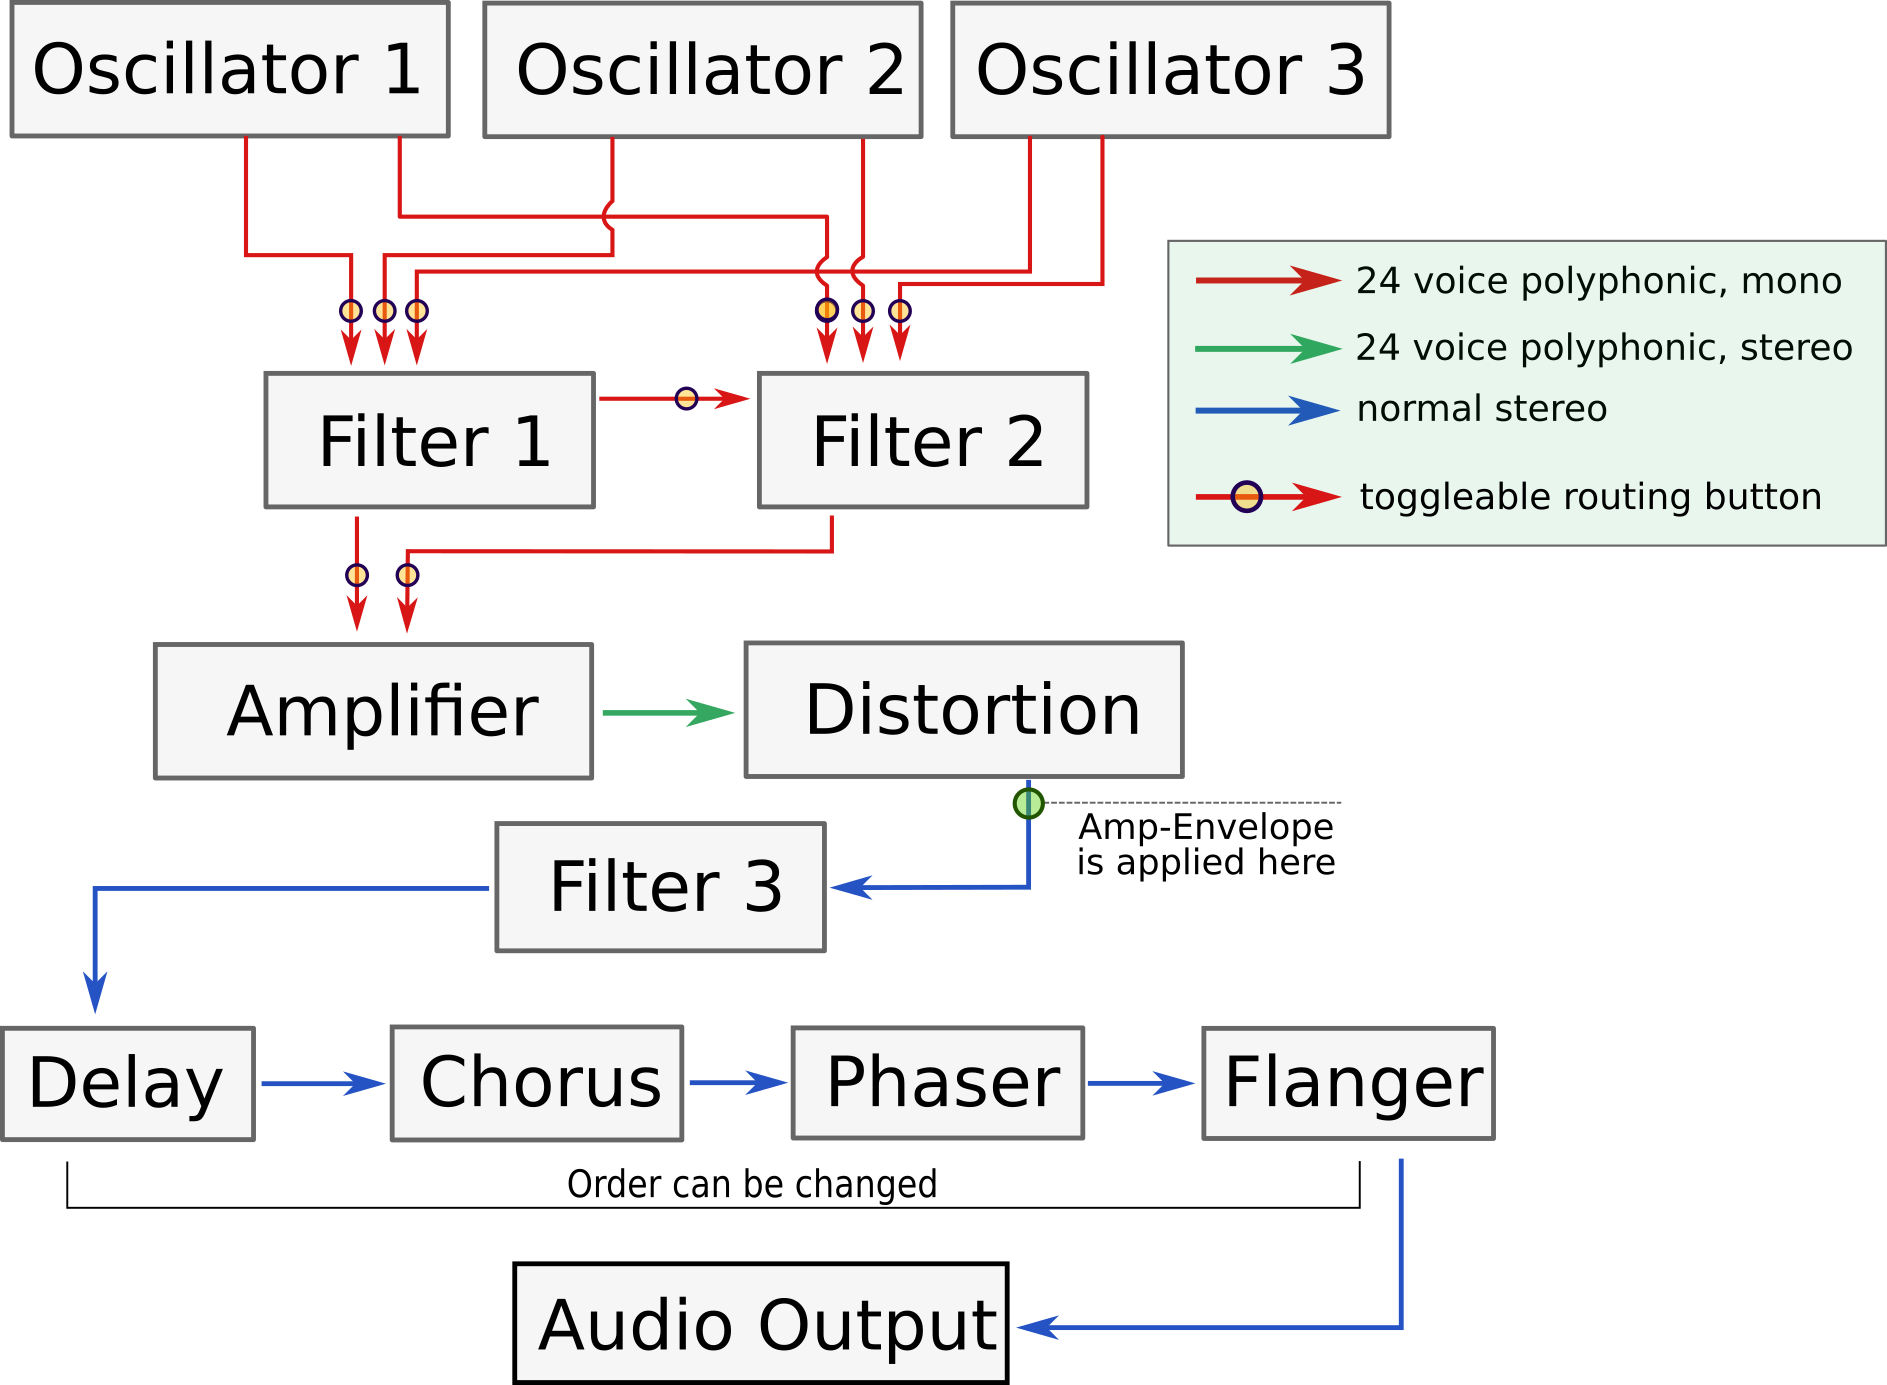
\includegraphics[width=\textwidth]{graphics/routing.png}
\end{center}


\vspace{1.5cm}
The routing buttons are located here on the GUI:
\begin{center}
    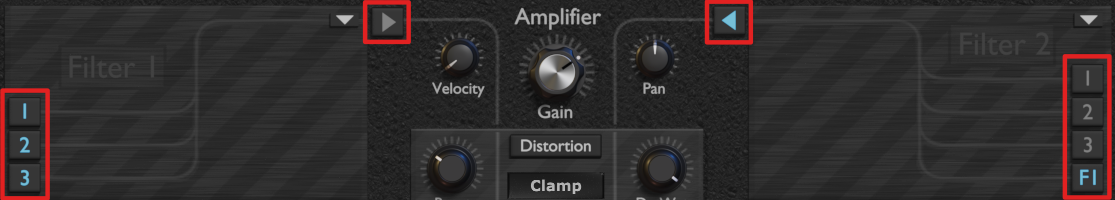
\includegraphics[width=\textwidth]{graphics/routing_buttons.png}
\end{center}

\audioparameter{Filter Input}{0}{1}{
    \begin{tabular}{L{0.1\textwidth} L{0.8\textwidth}}
        
        
\includegraphics[height=0.2\textwidth]{graphics/filter_input_buttons.png}
        &The buttons 1, 2 and 3 toggle the input of Oscillator 1, 2 and 3 into the Filter module. The button F1 is only available on Filter 2 and toggles the input of Filter 1 into Filter 2.
    \end{tabular}
}

\audioparameter{Filter Output}{0}{1}{
    \begin{tabular}{L{0.15\textwidth} L{0.8\textwidth}}
        
        
\includegraphics[width=0.13\textwidth]{graphics/filter_output_buttons.png}
        &These buttons toggle the output of the respective Filter modules into the Amplifier module.
    \end{tabular}
}

\vspace{5mm}
Per default, Odin 2 is set to \fat{serial processing}: All oscillators are routed into Filter 1, which is routed into Filter 2, which is routed into the Amplifier.

To use \fat{parallel processing}, enable "Filter 1 Output", Disable "Filter 2 Input F1" and input only the desired Oscillators into each Filter module.

\section{Scaling the Interface}
Odin 2 offers the possibility to scale the GUI to 100\% (800px $\times$ 614px) or 150\% (1200px $\times$ 921px). To do so, use the selector in the top right corner of the interface:
\begin{center}
    
\includegraphics[width=0.2\textwidth]{graphics/GUI_scaling.png}
\end{center}

\section{Help Inside the Plugin}
Maybe the most important feature to know in Odin 2 is the \fat{tooltip button}:

\begin{center}
    
\includegraphics[width=0.11\textwidth]{graphics/tooltip.png}
\end{center}

It is located in the top right corner of the GUI. When activated, you can \fat{hover over any parameter in the synth} and it will show you a tooltip, briefly describing its functionality.


\clearpage
\chapter{Oscillators}
Three oscillators form the basis of sound generation in Odin 2. You can choose from a wide variety of different modules, which are capable of wide palette of sounds, even without any further processing. Initially, Odin 2 starts out with an Analog Osc in slot 1 and none in slot 2 \& 3. You can change the module being used with the small dropdown button on the top-right of the osc-module:
\vspace{5mm}

\noindent
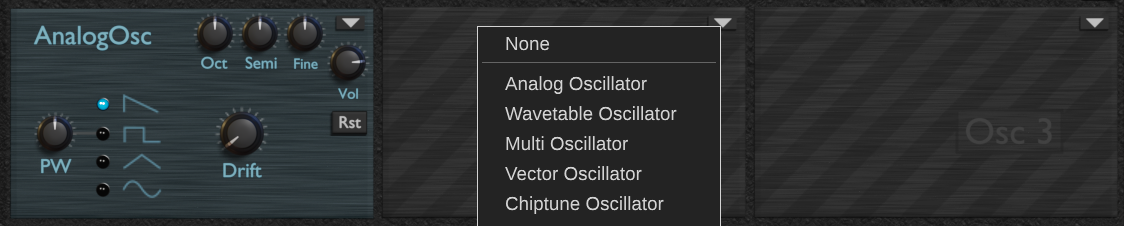
\includegraphics[width=\textwidth]{graphics/osc_selection.png}

\section{Common Parameters}
There are some controls which are common to all oscillator modules:

\audioparameterint{Osc Octave}
Detunes the oscillator by whole octaves.

\audioparameter{Osc Semitones}
Detunes the oscillator by semitones.

\audioparameter{Osc Finetune}
Detunes the oscillator by cents.

\audioparameter{Osc Volume}
Regulates the volume of this oscillator in deciBels. Can be used to shut the oscillator entirely. Modulating this parameter from the \modmatrix  works


\clearpage
\chapter{Filters}

\label{filters}
Signal filters are one of the basic tools to shape your sound in subtractive synthesis. While the oscillators in Odin 2 are already capable of a wide array of sounds, unprocessed oscillators usually sound very sharp and not pleasing to the ears. So what is a filter? A filter selectively removes frequencies from the spectrum, usually with some dials for the user to control the roll-off. Filters can be characterized by their frequency response, which tells us which frequencies are being attenuated or boosted:

\vspace{5mm}
\begin{center}
    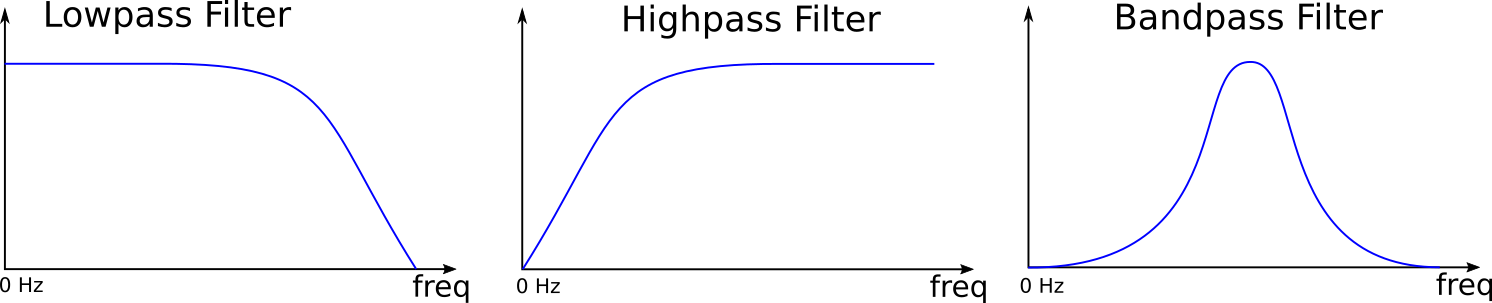
\includegraphics[width=\textwidth]{graphics/filter.png}
\end{center}

\vspace{5mm}

Odin 2 has three slots for filters which can be filled with a extensive selection of modules to shape your sound. A wide array of high quality virtual analog filter emulations is available, which emulate various analog filter circuits from synthesizer history.

\audioparameter{Filter Type}{0}{0}{To change the filter module, use the dropdown to the top-right of the filter module:

    \vspace{5mm}
    \begin{center}
        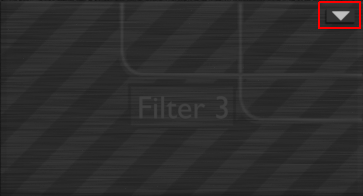
\includegraphics[width=0.5\textwidth]{graphics/filter_dropdown.png}
    \end{center}
}

\section{Common Controls}
Some of the controls are shared among most filter modules:

\begin{center}
    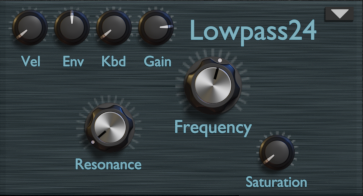
\includegraphics[width=0.5\textwidth]{graphics/lowpass_filter.png}
\end{center}

\audioparameter{Filter Frequency}{1}{1}
{Controls the cutoff point of the filter. The frequency value marks the point where the frequency is attenuated by 3dB.

    \begin{center}
        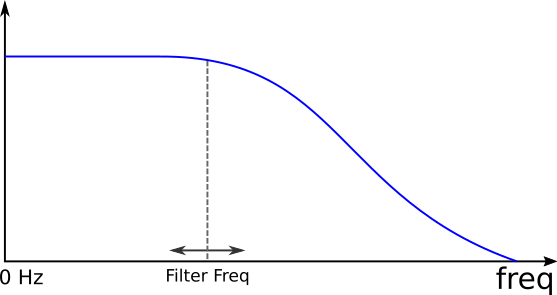
\includegraphics[width=0.5\textwidth]{graphics/filter_freq.png}
    \end{center}
}

\audioparameter{Filter Resonance}{1}{1}
{Increasing resonance creates a peak in the spectrum at the position of the filter cutoff.

    \begin{center}
        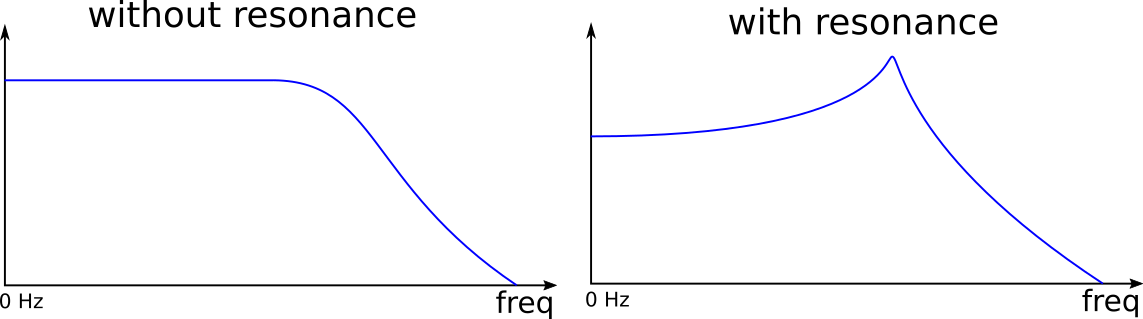
\includegraphics[width=0.9\textwidth]{graphics/filter_resonance.png}
    \end{center}

    Note also that the frequencies which were previously unaffected by the filter are being attenuated by the resonance parameter.

    None of the filters in Odin 2 are capable of self-oscillation for the sake of your ears and speakers.}

\audioparameter{Filter Velocity (Vel)}{1}{1}
{Adds velocity from MIDI-Notes to the filter frequency. This allows for expressive play, as harder key-hits move the filter freq up. Note that the value is added on top of the current value, so to achieve a similar resulting timbre, you might need to lower the filter frequency accordingly.}

\audioparameter{Filter Envelope (Env)}{1}{1}
{Controls the amount of Filter Envelope which is applied to the filter frequency. To see how the Filter Envelope itself is operated, see section \ref{ADSR}.}

\audioparameter{Filter Keyboard (Kbd)}{1}{1}
{Controls how much the MIDI-note is put on top of the filter frequency. Increasing this value makes the filter open up more for higher notes. This allows for more consistent notes across the keyboard, since higher notes might need higher filter freqs as well. Note that the value is added on top of the current value, so to achieve a similar resulting timbre, you might need to lower the filter frequency accordingly.}

\audioparameter{Filter Gain}{1}{1}
{Regulates the volume of this filter in deciBels. Can be used to shut the filter entirely. Modulating this parameter from the \modmatrix  with $-100$ will always shut the sound. Modulating this parameter with $+100$ will raise the sound to 0dB if the current value is smaller than -12dB. If it is bigger than -12dB, it will modulate to +12dB from the current value.}

\audioparameter{Filter Saturation}{1}{1}
{Introduces a slight distortion by shaping the signal with a hyperbolic tangent function. Depending on the filter module being used, the saturation stage is in a different position of the signal loop, yielding different results.}

\section{Lowpass, Bandpass, Highpass}
\begin{center}
    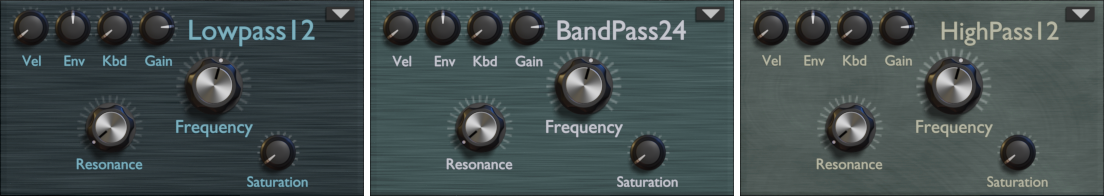
\includegraphics[width=\textwidth]{graphics/lp_bp_hp.png}
\end{center}

The staples of sound-design in Odin 2. These filters are virtual analog emulations of a certain, famous \fat{ladder filter} which has had a big impact in the history of synthesizers.

Each of these filters is available in a 12dB/Oct and a 24dB/Oct variant. These values determine the slope of the filter roll-off. The 24dB/Oct variants filter more frequencies than the 12dB/Oct counterparts.

\section{SEM-12}
\begin{center}
    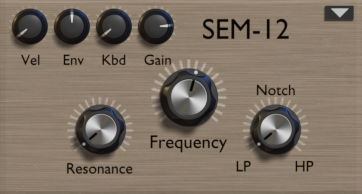
\includegraphics[width=0.5\textwidth]{graphics/SEM_filter.png}
\end{center}

Another emulation of a classic synthesizer filter. This filter has the specialty of being able to shift between a lowpass and a highpass filter, with a notch-filter in between. The filter slope of this filter is 12dB/Oct.

\audioparameter{SEM Transition}{1}{1}
{Fades from a lowpass filter over a notch filter to a highpass filter. This allows for special filter variants which still leave some of the frequencies that were filtered before.

    \begin{center}
        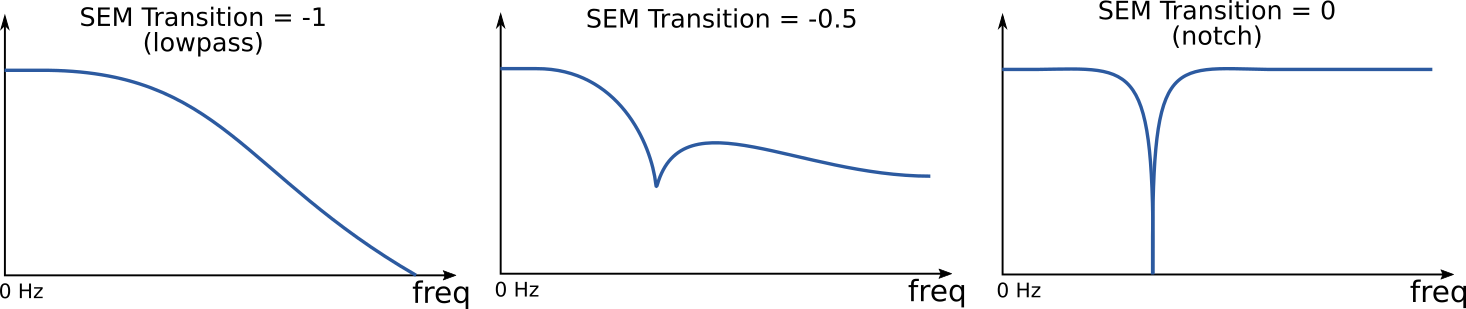
\includegraphics[width=\textwidth]{graphics/SEM_transition.png}
    \end{center}
}

\section{Diode Ladder}
\begin{center}
    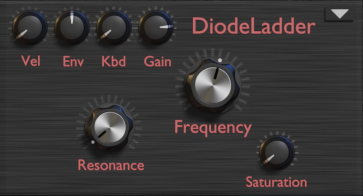
\includegraphics[width=0.5\textwidth]{graphics/diode_filter.png}
\end{center}

The Diode Ladder is a virtual analog emulation of another classic analog synthesizer filter. Its analog pendant was originally developed to work around a patent on the well established ladder filter. While still being 24dB/Oct, the characteristic of this filter is said to be more aggressive and wild compared to the classic ladder, especially when invoking resonance.

\section{KRG-35 LP / HP}
\begin{center}
    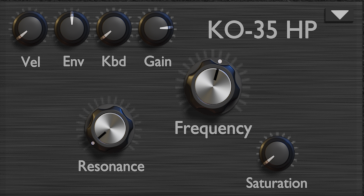
\includegraphics[width=0.5\textwidth]{graphics/korg_filter.png}
\end{center}

Yet another virtual analog emulation of one of the legendary analog filters of the past. This filter comes in a lowpass and highpass variant. Cranking up the resonance on these filters reveals a dirty, aggressive sound. Note that while the filters are named KRG-35, their slope is 12dB/Oct.

\section{Comb Filter}
\label{comb_filter}
\begin{center}
    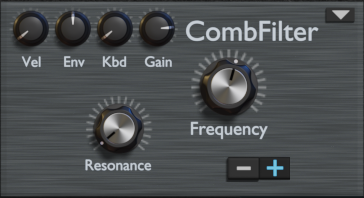
\includegraphics[width=0.5\textwidth]{graphics/comb_filter.png}
\end{center}

A comb filter is essentially a tuned \hyperref[delay]{delay module}. The input signal fed into a delay-line, which echos the sound back after a set amount of time. The delay time is the inverse of the filter frequency:

\begin{equation}
    t_{delay} = \frac{1}{f_{freq}}
\end{equation}

The frequency response of this filter usually resembles the shape of a hair-comb, hence the name.
\begin{center}
    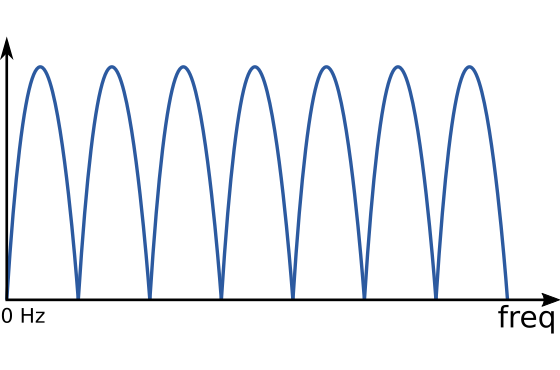
\includegraphics[width=0.5\textwidth]{graphics/comb_response.png}
\end{center}

The resonance parameter for the Comb Filter controls how much of the delayed signal is fed back into the delay line again, creating a feedback loop.

Comb filters can sound from subtle to metallic. When automating or modulating the frequency with high resonance values, a psychedelic smearing effect can be produced.

\audioparameter{Comb Polarity (+/-)}{0}{1}{
    Controls whether the insertion of the signal into the delay line is positive (+) or inverted (-). This changes the frequency behaviour. Inverted operation tends to eliminate deep frequencies.
}

\section{Formant Filter}
\begin{center}
    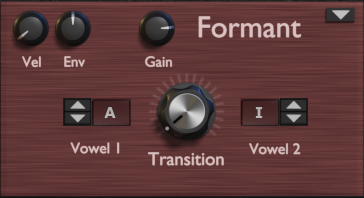
\includegraphics[width=0.5\textwidth]{graphics/formant_filter.png}
\end{center}
The Formant Filter tries to emulate vowels as they are produced in human speech. A tone is perceived as a vowel if two characteristic frequencies are dominant. These are called formants. The Formant Filter emulates this by using a combination of two resonator filters, which increase the frequencies around the two formants.

\begin{center}
    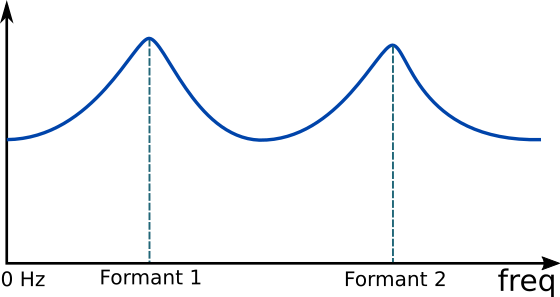
\includegraphics[width=0.5\textwidth]{graphics/formant_response.png}
\end{center}

The Formant Filter allows you to choose two vowels and freely move the formant peaks between the according formant peaks.

\audioparameter{Vowel 1 \& 2}{0}{0}{
    Select the vowels to the left and right of the transition. Selectable vowels are:

    A, E, I, O, U, \"A, \"O, \"U
}

\audioparameter{Formant Transition}{1}{1}{
    Transition between the two selected vowels. The transition is not a simple interpolation of the two vowel sounds, but actually moves the resonant formant peaks in the spectrum from one vowel to the next.

    The parameters Filter Velocity and Filter Envelope are applied to this parameter for the formant filter.
}

\section{Ring Modulator}
\begin{center}
    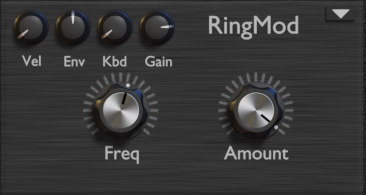
\includegraphics[width=0.5\textwidth]{graphics/ring_modulator.png}
\end{center}
The ring modulator is an oscillator disguised as a filter. The function of this module is to multiply the input signal with an internal sine-oscillator. This is formerly known as amplitude modulation.

\audioparameter{RingMod Freq}{1}{1}{
    Controls the frequency of the internal oscillator.
}

\audioparameter{RingMod Amount}{1}{1}{
    Controls the amount of ringmod to be applied. This interpolates between the input signal and the processed signal, effectively working like a Dry/Wet control.
}


\clearpage
\chapter{Amplifier \& Distortion}

\begin{center}
    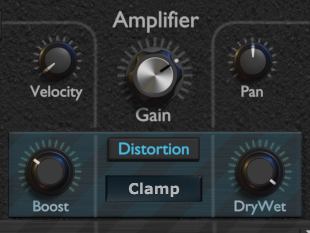
\includegraphics[width=0.4\textwidth]{graphics/amp_distortion.png}
\end{center}

The Amplifier and Distortion sections form the only parts in the signal flow in Odin 2 which are both polyphonic and stereo. 

\section{Amplifier}
\label{amplifier}

The amplifier section plays an important gain-staging role in odin. The sound can be boosted or attenuated, as well as panned.

\audioparameter{Amp Gain}{1}{1}{
    Changes the volume in in deciBels. Can be used to shut the sound entirely. Modulating this parameter from the \modmatrix  with $-100$ will always shut the sound. Modulating this parameter with $+100$ will raise the sound to 0dB if the current value is smaller than -12dB. If it is bigger than -12dB, it will modulate to +12dB from the current value.
}

\audioparameter{Amp Pan}{1}{1}{
    Pan or Panorama can be used to move the sound over the stereo field. The default value of zero will leave the sound centered. Moving the pan towards -1 will attenuate the right stereo channel, moving towards 1 does the same for the left channel.

    \begin{center}
        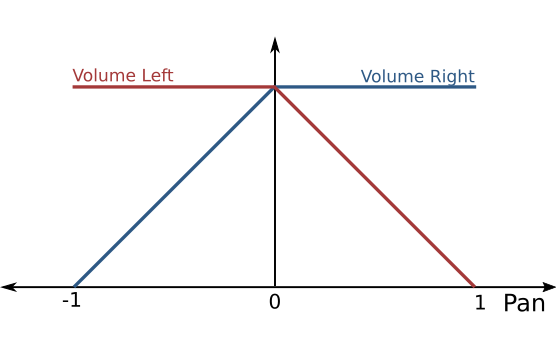
\includegraphics[width=0.7\textwidth]{graphics/pan_function.png}
    \end{center}
}

\audioparameter{Amp Velocity}{0}{1}{
    Makes the Amplifier gain sensible to the MIDI-Velocity. This allows for expressive play, where harder notes produce louder sounds. Increasing this value lowers the default gain of the amp, such that a MIDI-note with maximum velocity (127) will bring the level back to its previous level.
}

\begin{tcolorbox}[colback=yellow!10!white,
    colframe=white!20!black,
    center,
    valign=top,
    halign=left,
    center title,
    width=\textwidth]

Please note that the \hyperref[amp_env]{Amp Envelope} is not applied between the Amplifier and Distortion section, like the routing would suggest. The Amp Envelope is applied \fat{after the Distortion section}.
\end{tcolorbox}

\section{Distortion}
\label{distortion}

The Distortion module is capable of distorting the sound by various characteristic distortion functions. All the distortion types used in this section are threshold based: Once the wave surpasses a predefined value (in positive or negative direction), the processing will apply. Internally, 3x oversampling is used to prevent aliasing from the sharp cuts made to the waveform.

\audioparameter{Distortion On}{0}{1}{
    Turns the Distortion module on or off.
}

\vspace{20mm}
\audioparameter{Boost}{1}{1}{
    Boosts the gain of the incoming wave, making it surpass the internal threshold easier.
}

\vspace{20mm}
\audioparameter{Distortion DryWet}{1}{1}{
    Interpolates the processed and unprocessed signals, thereby controlling the amount of distortion applied to the sound.
}

\vspace{20mm}
\audioparameter{Distortion Algorithm}{0}{0}{
    Selects which distortion algorithm is used. The options are:
    
    \vspace{7mm}
    \fat{Clamp}: 
    Clamps the signal once it surpasses the threshold.

    \begin{center}
        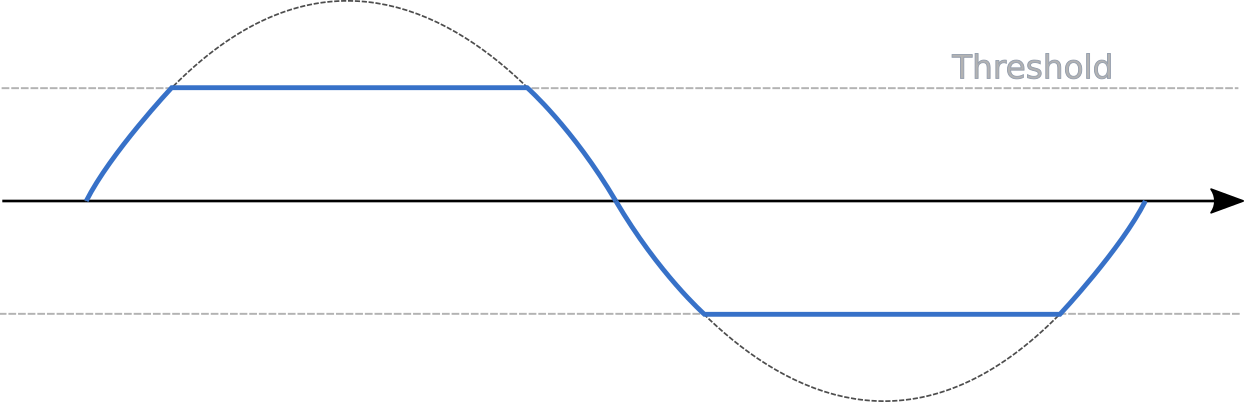
\includegraphics[width=0.7\textwidth]{graphics/overdrive.png}
    \end{center}

    \fat{Fold}: 
    Folds the wave over once it surpasses the threshold. If the folded wave hits the threshold on the other side, it will be folded again (and so on). Produces more harmonic content than the Clamp algorithm.

    \begin{center}
        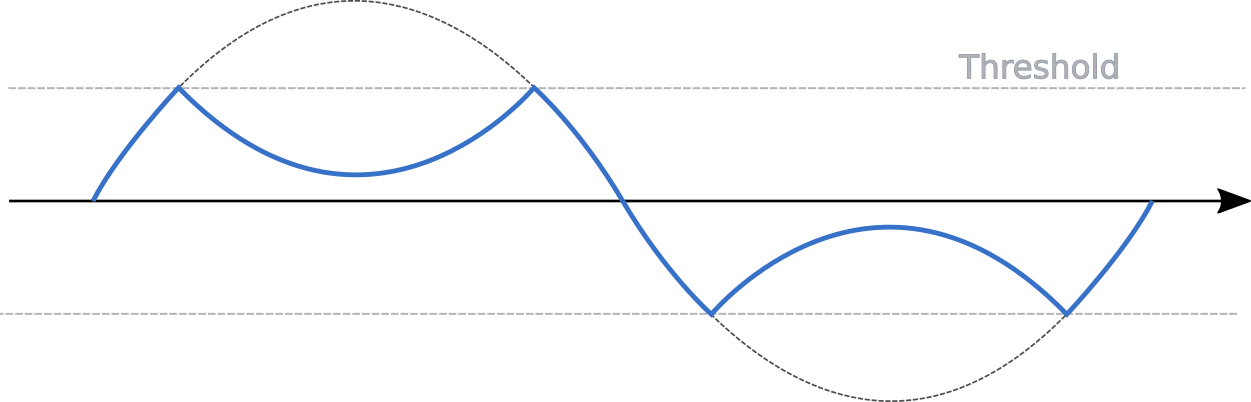
\includegraphics[width=0.7\textwidth]{graphics/fold.png}
    \end{center}

    \fat{Zero}: 
    Pulls the wave to zero once it surpasses the threshold. The strongest of the available distortion algorithms.

    \begin{center}
        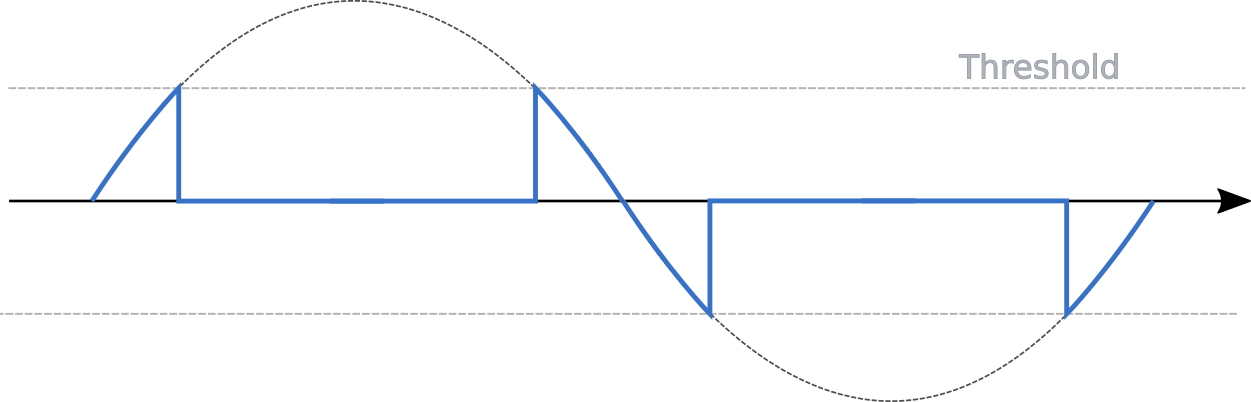
\includegraphics[width=0.7\textwidth]{graphics/zero.png}
    \end{center}
}

\clearpage
\chapter{FX}
\label{FX}
Odin 2 comes with five internal FX modules: \fat{Delay, Chorus, Phaser, Flanger} and \fat{Reverb}.

\begin{center}
    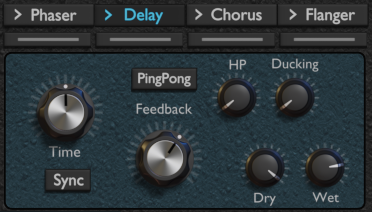
\includegraphics[width=0.4\textwidth]{graphics/FX.png}
\end{center}

The buttons on top of the FX modules serve multiple purposes:

\begin{center}
    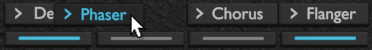
\includegraphics[width=0.4\textwidth]{graphics/FX_selector.png}
\end{center}

Clicking the corresponding name of the module reveals the corresponding module. The buttons below the module name are used to turn enable or disable the module.
You can also \fat{change the order of the modules}, by drag'n'dropping their name handles to the left or right.

\audioparameter{FX On}{0}{1}{
    Use the buttons below the module name to turn the FX module on or off. All modules can be used at the same time.
}

\audioparameter{FX Order}{0}{0}{
    Drag'n'drop the FX module handles to change the order of the FX. The algorithms are calculated in series from left to right.
}

\section{Delay}
\label{delay}
\begin{center}
    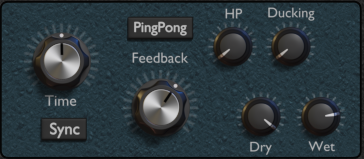
\includegraphics[width=0.5\textwidth]{graphics/delay.png}
\end{center}

A delay is a module capable of producing an 'echo' effect: The signal is fed into a delay-line, which outputs the signal again after a set amount of time again. The output of the delay line can also be fed back in, allowing a chain of attenuating echos. By controlling the delay time and feeback parameters, a wide variety of effects can be achieved. The Delay module in Odin 2 goes a step further and offers several additional features.

\audioparameter{Delay Time}{1}{1}{
    Controls the time the delay line takes to output the sound again. Depending on the parameter "Delay Sync", this is either a dial for continuous values in Hz, or a custom selector to sync the time to the beat. This selector allows for arbitrary fractions of the current host BPM, for example 5/16th notes:

    \begin{center}
        
\includegraphics[width=0.18\textwidth]{graphics/delay_sync.png}
    \end{center}
}

\audioparameter{Delay Feedback}{1}{1}{
    Controls how much of the output of the delay line is fed back in again. If feedback is zero, only one echo will be audible. If feedback is one, an infinite series of exact copies of sound will be output. Everything inbetween makes for slowly attenuating echos.
}

\audioparameter{Delay Sync}{0}{1}{
    Controls whether the Delay Time is set by a knob in Hz or via the sync-time selector, syncing it to the host BPM.
}

\audioparameter{Delay PingPong}{0}{1}{
    Enabling PingPong will make the left and right stereo delay lines crossfeed: The output of the left line is fed into the right line and vice versa.

    The initial input into the delay lines is mixed down to a mono signal and then fed into the left delay line only. The dry signal remains in the center of the stereo field.
}

\audioparameter{Delay Highpass (HP)}{1}{1}{
    The processed signal in the Delay module is filtered through a 6dB/Oct highpass filter. The Delay Highpass parameter controls the cutoff of this internal filter. This is great for removing the muddiness that deep frequencies can produce in a delay module.

    Note that the highpass filter is not applied inside, but after the feedback loop, i.e. consecutive echos do not get filtered further more as they are processed again.
}

\audioparameter{Ducking}{0}{1}{
    Ducking attenuates the output of the delayed signal if an input signal is present. This is great for decluttering sections where the delayed signal interferes with the unprocessed signal.
}

Unlike the other FX modules, the Delay features a separate Dry and Wet control to allow for easier adjustments of processed and unprocessed signals individually.
\audioparameter{Delay Dry}{1}{1}{
    Controls how much unprocessed signal is output by the Delay.
}

\audioparameter{Delay Wet}{1}{1}{
    Controls how much processed signal is output by the Delay.
}

\section{Chorus}
\begin{center}
    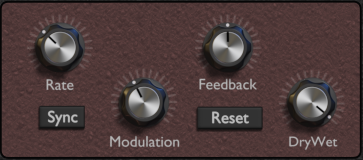
\includegraphics[width=0.5\textwidth]{graphics/chorus.png}
\end{center}

The Chorus module is a delay based effect capable of thickening sounds. The generated sound resembles that of a slightly detuned ensemble, hence the name chorus. Internally, the Chorus module uses a delay line, which is read from at two diferent positions. The delay times are modulated by an internal Low Frequency Oscillator (LFO). This slightly detunes the result resulting in the Chorus sound. The LFOs for the left and right channel are phase-offset by 90$^{\circ}$ to spread the sound in the stereo field.

\audioparameter{Chorus Rate}{1}{1}{
    Controls the speed of the internal LFO. Depending on the parameter "Chorus Sync", this is either a dial for continuous values in Hz, or a custom selector to sync the time to the beat. This selector allows for arbitrary fractions of the current host BPM, for example 5/16th notes:

    \begin{center}
        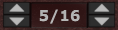
\includegraphics[width=0.18\textwidth]{graphics/chorus_sync.png}
    \end{center}
}

\audioparameter{Chorus Sync}{0}{1}{
    Controls whether the Chorus Rate is set by a knob in Hz or via the sync-time selector, syncing it to the host BPM.
}

\audioparameter{Chorus Modulation}{1}{1}{
    Controls how much the internal LFO modulates the two delay times. Exaggerates the detune effect.
}

\audioparameter{Chorus Feedback}{1}{1}{
    Controls how much of the output of the delay line is fed back in again. Pronounces the effect of the Chorus a bit more.
}

\audioparameter{Chorus DryWet}{1}{1}{
    Interpolates the processed and unprocessed signals, thereby controlling the strength of the effect.
}

\section{Phaser}
\begin{center}
    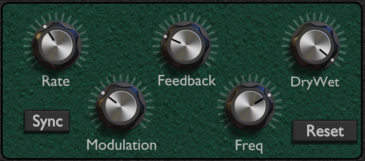
\includegraphics[width=0.5\textwidth]{graphics/phaser.png}
\end{center}
The phaser module introduces movement to the sound by applying a subtle "windy" character. The internal structure consists of a series of allpass filters: These filters do not alter the amplitude like the filters from Chapter \ref{filters}, but only shifts the phase of some frequencies. By adding the phase-shifted signal back onto the original signal, some of the frequencies get boosted, attenuated or eliminated entirely via phase-cancellation. The characteristic of the allpass-filters is continuously modulated by an internal Low Frequency Oscillator (LFO), which makes for the movemnet in the sound. The LFOs for the left and right channel are phase-offset by 90$^{\circ}$ to spread the sound in the stereo field.

\audioparameter{Phaser Rate}{1}{1}{
    Controls the speed of the internal LFO. Depending on the parameter "Phaser Sync", this is either a dial for continuous values in Hz, or a custom selector to sync the time to the beat. This selector allows for arbitrary fractions of the current host BPM, for example 5/16th notes:

    \begin{center}
        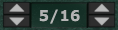
\includegraphics[width=0.18\textwidth]{graphics/phaser_sync.png}
    \end{center}
}

\audioparameter{Phaser Sync}{0}{1}{
    Controls whether the Phaser Rate is set by a knob in Hz or via the sync-time selector, syncing it to the host BPM.
}

\audioparameter{Phaser Modulation}{1}{1}{
    Controls how much the internal LFO modulates the internal allpass filters.
}

\audioparameter{Phaser Feedback}{1}{1}{
    An extra feedback stage, which feeds the output signal into the input again.
}

\audioparameter{Phaser Freq}{1}{1}{
    Shifts the base frequency of the internal allpass filters, thereby altering the characteristic of the effect.
}

\audioparameter{Phaser DryWet}{1}{1}{
    Controls how much of the phase-shifted signal is added to the input signal, thereby controling the strength of the effect.
}

\section{Flanger}
\begin{center}
    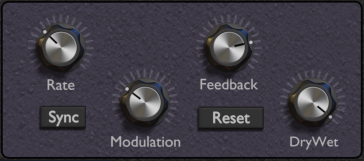
\includegraphics[width=0.5\textwidth]{graphics/flanger.png}
\end{center}

A Flanger is a modulated \hyperref[comb_filter]{comb filter}. The signal is fed into a delay line and mixed with the input signal after a small echo. The timing of this effect is modulated by an internal Low Frequency Oscillator (LFO). Additionally, the output of the delay line can be fed in again via the Feedback parameter, to allow for a continuous stream of echoes. The delay times for Comb Filters and Flangers is very short, usually below 50ms. 

\audioparameter{Flanger Rate}{1}{1}{
    Controls the speed of the internal LFO. Depending on the parameter "Flanger Sync", this is either a dial for continuous values in Hz, or a custom selector to sync the time to the beat. This selector allows for arbitrary fractions of the current host BPM, for example 5/16th notes:

    \begin{center}
        
\includegraphics[width=0.18\textwidth]{graphics/flanger_sync.png}
    \end{center}
}

\audioparameter{Flanger Sync}{0}{1}{
    Controls whether the Flanger Rate is set by a knob in Hz or via the sync-time selector, syncing it to the host BPM.
}

\audioparameter{Flanger Modulation}{1}{1}{
    Controls how much the internal LFO modulates the delay time.
}

\audioparameter{Flanger Feedback}{1}{1}{
    Controls how much of the output of the delay line is fed back in again. Creates a metallic smearing effect for big values. This parameter can be positive or negative allowing for positive and negative comb operation.
}

\audioparameter{Flanger DryWet}{1}{1}{
    Interpolates the processed and unprocessed signals, thereby controlling the strength of the effect.
}


\section{Reverb}
\begin{center}
    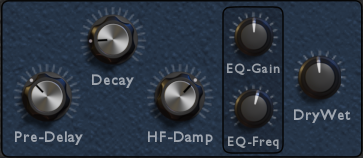
\includegraphics[width=0.5\textwidth]{graphics/reverb.png}
\end{center}

The reverb module provides a source of artificial reverberation in Odin 2. This module is sourced from \href{https://kokkinizita.linuxaudio.org/linuxaudio/zita-rev1-doc/quickguide.html}{Zita-rev1}. The reverb additionally features a built in equalizer with a rather large Q, to further shape the reverb to your hearts desire.

\audioparameter{Pre-Delay}{0}{1}{
    Controls how much the signal is delayed before being fed into the reverberation. This contributes to how big the emulated room feels.
}
\audioparameter{Decay}{0}{1}{
    Controls how fast the reverberation decays. The value in seconds controls the RT60, that is how long the signal takes to be attenuated by 60dB.
}
\audioparameter{HF-Damp}{0}{1}{
    Controls how much high frequencies are attenuated. Higher values will let more frequencies pass.
}
\audioparameter{EQ-Gain}{0}{1}{
    Controls the gain of the internal equalizer. The equalization will only be applied to the wet signal. Use this to highlight parts of the spectrum, or attenuate unwanted frequencies.
}
\audioparameter{EQ-Freq}{0}{1}{
    Controls the frequency of the internal equalizer. The equalization will only be applied to the wet signal. Use this to highlight parts of the spectrum, or attenuate unwanted frequencies.
}
\audioparameter{DryWet}{0}{1}{
    Controls the mix of unprocessed and processed sound.
}
\clearpage
\chapter{Modulators}

\clearpage
\chapter{Modulation Matrix}
\label{chapter_matrix}


\begin{center}
    \includegraphics[width=0.9\textwidth]{graphics/modmatrix.png}
\end{center}

The modulation matrix is where the true power of Odin 2 lies. A large amount of parameters inside the synthesizer can be modulated by a large variety of modulators.

\section{Basic Operation}

It might look daunting at first with the amount of controls it has to offer, but in reality it is nine rows of the same controls:

\begin{center}
    \includegraphics[width=0.9\textwidth]{graphics/modmatrix_row.png}
\end{center}

\audioparameter{Modulation Source}{0}{0}{
    Sets up a source for the modulation. The source chosen in this slot will be controlling the parameter set by "Destination 1" and "Destination 2" by the amounts set by "Destination 1 Amount" and "Destination 2 Amount".

    For a list of available modulation sources, see Section \ref{mod_sources}.
}

\audioparameter{Modulation Destination 1}{0}{0}{
    Sets up a destination for the modulation. The source chosen in this slot will be controlled the source set in "Modulation Source" by the amount set by "Destination 1 Amount".

    For a list of available modulation destinations, see Section \ref{mod_destinations}.
}

\audioparameter{Modulation Destination 2}{0}{0}{
    An independent second modulation destination with identical features to "Modulation Destination 1". Destinations 1 and 2 do not interfere with one another in any way.
}

\audioparameter{Destination 1 Amount}{0}{0}{
    Controls how much the Source modulates Destination 1. Can be positive or negative.
}

\audioparameter{Destination 2 Amount}{0}{0}{
    Controls how much the Source modulates Destination 2. Can be positive or negative.
}

You can use the X-Buttons to the right of each row to instantaneously clear the entire modulation row.

\section{Modulation Scaling}

An advanced feature of the modulation matrix in Odin 2 is the "Modulation Scale" option. You can scale the modulation that was set up with the parameters above by another modulation source. The value of the source chosen for scale now controls the modulation depth. This way you can essentially modulate the modulation itself. A common use case for this includes scaling with the Modwheel: The set up modulation now can be controlled by the keyboard player by moving the Modwheel up and down.

\vspace{10mm}
Consider the following graphic: On the left side, an LFO is set up to modulate a parameter. On the right side, the modulation is scaled by another, slower moving LFO:
\begin{center}
    \includegraphics[width=\textwidth]{graphics/modulation_scale.png}
\end{center}
We can see how the actual modulation curve gets more complex instantaneously.

\audioparameter{Modulation Scale}{0}{0}{
    Select which modulation source is used to scale the modulations. Note that the scaling applies to Destination 1 and Destination 2 in the same way.

    For a list of available modulation sources, see Section \ref{mod_sources}.
}

\audioparameter{Scale Amount}{0}{0}{
    Determines the amount of scaling applied to the modulation. Using a scale amount of 100 is equivalent of multiplying the "Source" and "Scale" values together. For values between 0 and 100, linear interpolation logic applies between the raw modulation and and the multiplied values. For values below zero, the scaling source is inverted.
}

\section{Mono \& Poly Modulation}

Some of the modulation sources and destinations inside Odin 2 are polyphonic (i.e. exist once per voice), while others are monophonic (exist once per plugin instance). The following table summarizes the behavior when setting up poly/mono source and destination combos:

{\renewcommand{\arraystretch}{1.6}
\begin{tabular}{| L{0.2\textwidth} | L{0.35\textwidth} | L{0.35\textwidth} |}
    \hline
                                                              &
    \fat{Mono Destination}                                    &
    \fat{Poly Destination}                                      \\
    \hline
    \fat{Mono Source}                                         &
    single modulation source and destination                  &
    a single source modulates all destinations                  \\
    \hline
    \fat{Poly Source}                                         &
    only the most most recent voice modulates the destination &
    each voice is modulated independently                       \\
    \hline
\end{tabular}
}

\vspace{5mm}
A similar logic applies when dealing with poly/mono modulation scaling.

\vspace{5mm}
To see which modulations are poly or mono, refer to the tables in Section \ref{mod_sources} and Section \ref{mod_destinations}.

\section{Modulation Sources}
\label{mod_sources}
This list provides an overview over all modulation sources available in Odin 2:

Note that all unipolar sources operate in the range [0, 1], and all bipolar sources in the range [-1, 1].

\newcommand{\modsource}[4]{
    \fat{#1} &
    \IfEqCase{#2}{%
        {M}{Mono}%
            {P}{Poly}%
    }[\PackageError{audioparameter}{Undefined option to param: #2}{}]  &
    \IfEqCase{#3}{%
        {U}{Unipolar}%
            {B}{Bipolar}%
    }[\PackageError{audioparameter}{Undefined option to param: #3}{}] &
    #4 \\
    \hline
}

\vspace{5mm}
{\renewcommand{\arraystretch}{1.4}
    \begin{longtable}{| L{0.2\textwidth} | L{0.1\textwidth} | L{0.12\textwidth} |L{0.5\textwidth} |}
        \hline

        \fat{Source}     &
        \fat{Mono /Poly} &
        \fat{Polarity}   &
        \fat{Description}  \\
        \hline

        \modsource{Oscillator 1}{P}{B}{
            The output of the \hyperref[oscillators]{Oscillator} module that is currently in slot 1.
        }
        \modsource{Oscillator 2}{P}{B}{
            The output of the \hyperref[oscillators]{Oscillator} module that is currently in slot 2.
        }
        \modsource{Oscillator 3}{P}{B}{
            The output of the \hyperref[oscillators]{Oscillator} module that is currently in slot 3.
        }
        \modsource{Filter 1 Out}{P}{B}{
            The output of the \hyperref[filters]{Filter module} that is currently in slot 1. If no Filter is present, the bypassed signal is used.
        }
        \modsource{Filter 2 Out}{P}{B}{
            The output of the \hyperref[filters]{Filter module} that is currently in slot 2. If no Filter is present, the bypassed signal is used.
        }
        \modsource{Amp Envelope}{P}{U}{
            The \hyperref[ADSR]{Amplifier Envelope}.
        }
        \modsource{Filter Envelope}{P}{U}{
            The \hyperref[ADSR]{Filter Envelope}.
        }
        \modsource{Mod Envelope}{P}{U}{
            The \hyperref[ADSR]{Modulation Envelope}.
        }
        \modsource{Global Envelope}{M}{U}{
            The \hyperref[ADSR]{Global Envelope}.
        }
        \modsource{LFO 1}{P}{B}{
            The output of \hyperref[LFOs]{LFO 1}.
        }
        \modsource{LFO 2}{P}{B}{
            The output of \hyperref[LFOs]{LFO 2}.
        }
        \modsource{LFO 3}{P}{B}{
            The output of \hyperref[LFOs]{LFO 3}.
        }
        \modsource{Global LFO}{M}{B}{
            The output of the \hyperref[LFOs]{Global LFO}.
        }
        \modsource{X}{M}{U}{
            The X-coordinate of the \hyperref[xy]{XY-Pad}.
        }
        \modsource{Y}{M}{U}{
            The Y-coordinate of the \hyperref[xy]{XY-Pad}.
        }
        \modsource{Modwheel}{M}{U}{
            The position of the \hyperref[wheels]{Modwheel}.
        }
        \modsource{PitchBend}{M}{B}{
            The position of the \hyperref[wheels]{PitchBend wheel}.
        }
        \modsource{MIDI Note}{P}{U}{
            The index of the MIDI note-on event, scaled from 0 (note: 0, C-2) to 1 (note: 127, G8).
        }
        \modsource{MIDI Velocity}{P}{U}{
            The velocity of the MIDI note-on event, scaled from 0 (vel: 0) to 1 (vel: 127).
        }
        \modsource{Channel Pressure}{M}{U}{
            Often referred to as "Mono Aftertouch". A pressure value applied to the keyboard after pressing a key, scaled from 0 (CP: 0) to 1 (CP: 127).
        }
        \modsource{Unison Index}{P}{B}{
            A unique value for each voice in a \hyperref[unison]{unison voice cluster}. The value is the one that is used to spread the voices over the stereo field.
        }
        \modsource{Arp Mod 1}{P}{B}{
            The upper row of modulation parameters from the \hyperref[arpeggiator]{Arpeggiator module}. This value is distributed to the voice that is triggered by that sequence step.
        }
        \modsource{Arp Mod 2}{P}{B}{
            The lower row of modulation parameters from the \hyperref[arpeggiator]{Arpeggiator module}. This value is distributed to the voice that is triggered by that sequence step.
        }
        \modsource{Sustain Pedal}{M}{U}{
            The pedal that is commonly used on (digital) pianos to avoid releasing keys.
        }
        \modsource{Soft Pedal}{M}{U}{
            The pedal that is commonly used on (digital) pianos to attenuate the volume of keys.
        }
        \modsource{Random}{P}{B}{
            A random value that is generated every time a new voice is triggered
        }
        \modsource{Constant}{M}{U}{
            A constant value of 1
        }
    \end{longtable}
}


\section{Modulation Destinations}
\label{mod_destinations}

This is an overview of all available modulation destinations in Odin 2. The column "Range" describes the amount of modulation that is applied if you use a "Constant" source and modulate by an amount of +100 or -100. Note that most destinations have internal logical limits for their modulation ranges. For example, the "Amplifier Pan" can not get out of the range [-1, 1].

\newcommand{\moddest}[5]{
    \fat{#1} &
    \IfEqCase{#2}{%
        {M}{\scriptsize{Mono}}%
            {P}{\scriptsize{Poly}}%
    }[\PackageError{audioparameter}{Undefined option to param: #2}{}]  &
    \footnotesize{#3} &
    \footnotesize{\fat{+100}: #4}

    \footnotesize{\fat{-100}: #5}\\
    \hline
}

\newcommand{\moddestcategory}[1]{
    \multicolumn{4}{|c|}{\fat{#1}} \\
    \hline
}

{\renewcommand{\arraystretch}{1.4}
    \begin{longtable}{| L{0.15\textwidth}| L{0.05\textwidth} | L{0.34\textwidth} | L{0.37\textwidth}|}
        \hline

        \fat{Destination}             &
        \scriptsize{\fat{Mono/ Poly}} &
        \fat{Description}             &
        \fat{Range}                     \\
        \hline

        \moddestcategory{Oscillator Common}

        \moddest{Osc Pitch Exp}{P}{
            Exponential modulation of the oscillator pitch}{
            Two octaves up}{
            Two octaves down}
        \moddest{Osc Pitch Lin}{P}{
            Linear modulation of the oscillator pitch}{
            Adds two times the current frequency}{
            Subtracts two times the current frequency, making the oscillator run backwards.}
        \moddest{Osc Volume}{P}{
            Modulates the volume of the oscillator
        }{
            If the volume is below -12dB, then modulation is up to 0dB. If the volume is above -12dB, then modulation is 12dB up from that point.
        }{
            Modulates to $-\infty$dB.
        }

        \moddestcategory{Analog Osc}
        \moddest{Pulse Width}{P}{
            Modulates the pulse width of the pulse wave. Unlike the control knob, this can be used to achieve a pulse-width of 0\% or 100\% (no sound) and beyond.
        }{
            Increase duty cycle by 100\%
        }{
            Decrease duty cycle by 100\%
        }
        \moddestcategory{Wavetable / Multi Osc}
        \moddest{Osc Position}{P}{
            Modulates the position used for interpolating between the four subtables.
        }{
            Move once through the entire table.
        }{
            Move once through the entire table backwards.
        }
        \moddestcategory{Multi Osc}

        \moddest{Osc Detune}{P}{
            Modulates the detuning of the sub-oscillators.
        }{
            Same as moving the control knob by a value of +1.
        }{
            Same as moving the control knob by a value of -1.
        }
        \moddest{Osc Spread}{P}{
            Modulates the spreading of the sub-oscillators across the wavetable.
        }{
            Same as moving the control knob by a value of +1.
        }{
            Same as moving the control knob by a value of -1.
        }
        \moddestcategory{Vector Osc}
        \moddest{Osc X}{P}{
            Modulate the X position of the vector pad.
        }{
            Move the handle the width of the pad to the right.
        }{
            Move the handle the width of the pad to the left.
        }
        \moddest{Osc Y}{P}{
            Modulate the Y position of the vector pad.
        }{
            Move the handle the height of the pad up.
        }{
            Move the handle the height of the pad down.
        }
        \moddestcategory{Chiptune Osc}
        \moddest{Osc Arp Speed}{P}{
            Modulates the speed of the arpeggiator in the chiptune osc exponentially.
        }{
            Increase the speed by a factor of 4.
        }{
            Decrease the speed by a factor of $1/4$.
        }
        \moddestcategory{FM and PhaseMod Oscs}
        \moddest{Osc FM amount}{P}{
            Modulates the amount of frequency modulation between carrier and modulator oscs.
        }{
            Same as moving the control knob by a value of +1.
        }{
            Same as moving the control knob by a value of -1.
        }
        \moddest{Osc FM amount}{P}{
            Modulates the amount of phase modulation between carrier and modulator oscs.
        }{
            Same as moving the control knob by a value of +1.
        }{
            Same as moving the control knob by a value of -1.
        }
        \moddest{Modulator Ratio}{P}{
            Modulates the ratio used for the modulator (see Section \ref{fm_osc}). Unlike the controls, this can be used to generate irrational fractions.
        }{
            Increases the current ratio by a factor of four.
        }{
            Decrease the current ratio by a factor of $1/4$.
        }
        \moddest{Carrier Ratio}{P}{
            Modulates the ratio used for the carrier (see Section \ref{fm_osc}). Unlike the controls, this can be used to generate irrational fractions.
        }{
            Increases the current ratio by a factor of four.
        }{
            Decrease the current ratio by a factor of $1/4$.
        }
        \moddestcategory{Noise Osc}
        \moddest{Osc LP Frequency}{P}{
            Modulates the frequency of the lowpass filter in the noise osc exponentially.
        }{
            Modulates the frequency 64 semitones up (factor 40.317).
        }{
            Modulates the frequency 64 semitones down (factor 0.0248).
        }
        \moddest{Osc HP Frequency}{P}{
            Modulates the frequency of the highpass filter in the noise osc exponentially.
        }{
            Modulates the frequency 64 semitones up (factor 40.317).
        }{
            Modulates the frequency 64 semitones down (factor 0.0248).
        }
        \moddestcategory{Filter Common}
        \moddest{Filter Frequency}{P}{
            Modulates the filter frequency exponentially.
        }{
            Modulates the frequency 64 semitones up (factor 40.317).
        }{
            Modulates the frequency 64 semitones down (factor 0.0248).
        }
        \moddest{Filter Resonance}{P}{
            Modulates the resonance of the filter.
        }{
            Same as moving the control knob by a value of +1.
        }{
            Same as moving the control knob by a value of -1.
        }
        \moddest{Filter Gain}{P}{
            Modulates the volume of the filter.
        }{
            If the current gain is below -12dB, then modulation is up to 0dB. If the gain is above -12dB, then modulation is 12dB up from that point.
        }{
            Modulates to $-\infty$dB.
        }
        \moddest{Filter Env Amount}{P}{
            Modulates how much envelope is applied to the filter.
        }{
            Same as moving the control knob by a value of +1.
        }{
            Same as moving the control knob by a value of -1.
        }
        \moddest{Filter Vel Amount}{P}{
            Modulates the velocity sensitivity of the filter.
        }{
            Same as moving the control knob by a value of +1.
        }{
            Same as moving the control knob by a value of -1.
        }
        \moddest{Filter Kbd Amount}{P}{
            Modulates the keyboard sensitivity of the filter.
        }{
            Same as moving the control knob by a value of +1.
        }{
            Same as moving the control knob by a value of -1.
        }
        \moddest{Filter Saturation}{P}{
            Modulates the saturation of the filter.
        }{
            Same as moving the control knob by a value of +1.
        }{
            Same as moving the control knob by a value of -1.
        }
        \moddestcategory{SEM-12 Filter}
        \moddest{Filter SEM Transition}{P}{
            Modulates the filter characteristic transition from lowpass over notch to highpass.
        }{
            Same as moving the control knob by a value of +1.
        }{
            Same as moving the control knob by a value of -1.
        }
        \moddestcategory{Formant Filter}
        \moddest{Filter Formant Transition}{P}{
            Modulates the transition from the left vowel to the right.
        }{
            Same as moving the control knob by a value of +1.
        }{
            Same as moving the control knob by a value of -1.
        }
        \moddestcategory{Amplifier}
        \moddest{Amplifier Gain}{P}{
            Modulates the gain in the Amplifier module.
        }{
            If the current gain is below -12dB, then modulation is up to 0dB. If the gain is above -12dB, then modulation is 12dB up from that point.
        }{
            Modulates to $-\infty$dB.
        }
        \moddest{Amplifier Pan}{P}{
            Modulates the position of the sound in the stereo field.
        }{
            Same as moving the control knob by a value of +1.
        }{
            Same as moving the control knob by a value of -1.
        }
        \moddestcategory{Distortion}
        \moddest{Distortion Boost}{P}{
            Modulates the input boost of the distortion module.
        }{
            Same as moving the control knob by a value of +1.
        }{
            Same as moving the control knob by a value of -1.
        }
        \moddest{Distortion DryWet}{P}{
            Modulates the relation of unprocessed and processed signal in the Distortion module.
        }{
            Same as moving the control knob by a value of +1.
        }{
            Same as moving the control knob by a value of -1.
        }
        \moddestcategory{ADSR Envelopes}
        \moddest{Env Attack}{P}{
            Modulates the attack time of the Envelope exponentially and linearly. This parameter is Mono for the Global Env.
        }{
            Scales the current time by a factor of 8 and then adds 0.3 seconds.
        }{
            Scales the current time by a factor of $1/8$ and then subtracts 0.3 seconds.
        }
        \moddest{Env Decay}{P}{
            Modulates the decay time of the Envelope exponentially and linearly. This parameter is Mono for the Global Env.
        }{
            Scales the current time by a factor of 8 and then adds 0.3 seconds.
        }{
            Scales the current time by a factor of $1/8$ and then subtracts 0.3 seconds.
        }
        \moddest{Env Sustain}{P}{
            Modulates the sustain value of the Envelope.
        }{
            Same as moving the control slider +1.
        }{
            Same as moving the control slider -1.
        }
        \moddest{Env Release}{P}{
            Modulates the release time of the Envelope exponentially and linearly. This parameter is Mono for the Global Env.
        }{
            Scales the current time by a factor of 8 and then adds 0.3 seconds.
        }{
            Scales the current time by a factor of $1/8$ and then subtracts 0.3 seconds.
        }
        \moddestcategory{LFOs}
        \moddest{LFO Freq}{P}{
            Modulates the frequency of the LFO exponentially. This parameter is Mono for the Global LFO.
        }{
            Increases current frequency by 4 octaves (factor 16).
        }{
            Decreases current frequency by 4 octaves (factor 0.0625).
        }
        \moddestcategory{Delay}
        \moddest{Delay Time}{M}{
            Modulates the delay time exponentially.
        }{
            Increases the current time by a factor of 3.
        }{
            Decreases the current time by a factor of $1/3$.
        }
        \moddest{Delay Feedback}{M}{
            Modulates the feedback of the delay line.
        }{
            Same as moving the control knob by a value of +1.
        }{
            Same as moving the control knob by a value of -1.
        }
        \moddest{Delay HP Freq}{M}{
            Modulates the frequency of the highpass filter in the Delay module exponentially.
        }{
            Modulates the frequency 64 semitones up (factor 40.317).
        }{
            Modulates the frequency 64 semitones down (factor 0.0248).
        }
        \moddest{Delay Dry}{M}{
            Modulates the output of unprocessed signal from the Delay module.
        }{
            Same as moving the control knob by a value of +1.
        }{
            Same as moving the control knob by a value of -1.
        }
        \moddest{Delay Wet}{M}{
            Modulates the output of processed signal from the Delay module.
        }{
            Same as moving the control knob by a value of +1.
        }{
            Same as moving the control knob by a value of -1.
        }
        \moddestcategory{Phaser}
        \moddest{Phaser Rate}{M}{
            Modulates the speed of the internal LFO exponentially.
        }{
            Increases the speed by a factor of 4.
        }{
            Decreases the speed by a factor of $1/4$.
        }
        \moddest{Phaser Amount}{M}{
            Modulates the depth of frequency modulation by the LFO in the Phaser.
        }{
            Same as moving the control knob by a value of +1.
        }{
            Same as moving the control knob by a value of -1.
        }
        \moddest{Phaser Freq}{M}{
            Modulates the base frequency of the internal allpass filters linearly.
        }{
            Moves the frequency up 2000Hz.
        }{
            Moves the frequency down 2000Hz.
        }
        \moddest{Phaser Feedback}{M}{
            Modulates the internal feedback of the Phaser module.
        }{
            Same as moving the control knob by a value of +1.
        }{
            Same as moving the control knob by a value of -1.
        }
        \moddest{Phaser Drywet}{M}{
            Modulates the ratio of processed and unprocess signals output by the Phaser module.
        }{
            Same as moving the control knob by a value of +1.
        }{
            Same as moving the control knob by a value of -1.
        }
        \moddestcategory{Chorus}
        \moddest{Chorus Rate}{M}{
            Modulates the speed of the internal LFO exponentially.
        }{
            Increases the speed by a factor of 4.
        }{
            Decreases the speed by a factor of $1/4$.
        }
        \moddest{Chorus Amount}{M}{
            Modulates the depth of frequency modulation by the LFO in the Chorus.
        }{
            Same as moving the control knob by a value of +1.
        }{
            Same as moving the control knob by a value of -1.
        }
        \moddest{Chorus Feedback}{M}{
            Modulates the feedback of the internal delay line.
        }{
            Same as moving the control knob by a value of +1.
        }{
            Same as moving the control knob by a value of -1.
        }
        \moddest{Chorus Drywet}{M}{
            Modulates the ratio of processed and unprocess signals output by the Chorus module.
        }{
            Same as moving the control knob by a value of +1.
        }{
            Same as moving the control knob by a value of -1.
        }
        \moddestcategory{Flanger}
        \moddest{Flanger Rate}{M}{
            Modulates the speed of the internal LFO exponentially.
        }{
            Increases the speed by a factor of 4.
        }{
            Decreases the speed by a factor of $1/4$.
        }
        \moddest{Flanger Amount}{M}{
            Modulates the depth of frequency modulation by the LFO in the Flanger.
        }{
            Same as moving the control knob by a value of +1.
        }{
            Same as moving the control knob by a value of -1.
        }
        \moddest{Flanger Feedback}{M}{
            Modulates the feedback of the internal delay line.
        }{
            Same as moving the control knob by a value of +1.
        }{
            Same as moving the control knob by a value of -1.
        }
        \moddest{Flanger Drywet}{M}{
            Modulates the ratio of processed and unprocess signals output by the Flanger module.
        }{
            Same as moving the control knob by a value of +1.
        }{
            Same as moving the control knob by a value of -1.
        }
        \moddestcategory{Arpeggiator}
        \moddest{Arp Speed}{M}{
            Modulates the speed of the Arpeggiator module exponentially
        }{
            Doubles the speed.
        }{
            Halves the speed.
        }
        \moddest{Arp Gate}{M}{
            Modulates the gate time in the Arpeggiator module.
        }{
            Adds 100\% gate time.
        }{
            Subtracts 100\% gate time.
        }
        \moddestcategory{XY-Pad}
        \moddest{XY-Pad X}{M}{
            Modulates X coordinate of the XY-Pad in the synth (see Section \ref{xy}).
        }{
            Like moving the handle once across the pad to the right.
        }{
            Like moving the handle once across the pad to the left.
        }
        \moddest{XY-Pad Y}{M}{
            Modulates Y coordinate of the XY-Pad in the synth (see Section \ref{xy}).
        }{
            Like moving the handle once across the pad upwards.
        }{
            Like moving the handle once across the pad downwards.
        }
        \moddestcategory{Global}
        \moddest{Glide}{M}{
            Modulates the Glide parameter in the synth (see Section \ref{glide}).
        }{
            Same as moving the control knob by a value of +1.
        }{
            Same as moving the control knob by a value of -1.
        }
        \moddest{Master}{M}{
            Modulates the master gain of the synthesizer.
        }{
            If the current master gain is below -12dB, then modulation is up to 0dB. If the master gain is above -12dB, then modulation is 12dB up from that point.
        }{
            Modulates to $-\infty$dB.
        }
    \end{longtable}
}
\clearpage
\chapter{Arpeggiator \& Step Sequencer}
\label{arpeggiator}

\begin{center}
    \includegraphics[width=\textwidth]{graphics/arpeggiator.png}
\end{center}

The Arpeggiator \& Step Sequencer is a tool which is able to automatically play complex rhytmic sequences from a given set of input notes. Activating this module overrides the notes you're inputting into the synthesizer and generates note sequences itself.

\begin{tcolorbox}[colback=yellow!10!white,
    colframe=white!20!black,
    center,
    valign=top,
    halign=left,
    center title,
    width=\textwidth]

    The Arpeggiator \& Step Sequencer occupies the same space in the GUI as the modulation matrix and the Preset Library. If you can't locate the module in the lower right corner of the GUI, press the "Arpeggiator" button above the modulation matrix:

    \begin{center}
        \includegraphics[width=\textwidth]{graphics/arpeggiator_button.png}
    \end{center}
\end{tcolorbox}

The basic operation of this module is to listen for the inputs you play on the keyboard and play them over a set of octaves. You can control various parameters, like the amount of octaves, the direction of the arpeggio, gate length, which notes to omit and many more.

\audioparameter{Arpeggiator On}{0}{1}{
    \begin{center}
        \includegraphics[height=0.08\textwidth]{graphics/arpeggiator_on.png}
    \end{center}    

    Turns the Arpeggiator \& Step Sequencer module on or off.
}

\audioparameter{Arpeggiator Step Time}{1}{0}{
    \begin{center}
        \includegraphics[width=0.17\textwidth]{graphics/arpeggiator_speed.png}
    \end{center}
    Controls the time one step takes, synced to the host BPM. The image above represents a length of $2/16$th or $1/8$th note. This parameter can be modulated in the \modmatrix to achieve non-synced values.
}

\audioparameter{Arpeggiator Octaves}{0}{0}{
    \begin{center}
        \includegraphics[width=0.17\textwidth]{graphics/arpeggiator_octaves.png}
    \end{center}
    Controls over how many octaves the arpeggio will be played. For a pure Step Sequencer style operation, set this value to 1.
}

\audioparameter{Arpeggiator Gate Length}{1}{0}{
    \begin{center}
        \includegraphics[width=0.17\textwidth]{graphics/arpeggiator_gate.png}
    \end{center}
    Controls how long a note is played, before a note-off signal is sent to the synthesizer. The times are represented in percent of the current step time. If the gate length is bigger than 100\%, each step will overlap into the next step.
}


\audioparameter{Arpeggiator Direction}{0}{0}{
    \begin{center}
        \includegraphics[width=0.17\textwidth]{graphics/arpeggiator_direction.png}
    \end{center}

    Determines the play style of the arpeggiator. The resulting notes for the various directions will be displayed here for "Arpeggiator Octaves" set to 2, Speed of $1/16$ and a C-major chord as an input:

    \begin{center}
        \includegraphics[height=0.08\textwidth]{graphics/c_major.png}
    \end{center}

    \fat{Direction: Up}
    \begin{center}
        \includegraphics[height=0.08\textwidth]{graphics/arpeggiator_up.png}
    \end{center}

    \fat{Direction: Down}
    \begin{center}
        \includegraphics[height=0.08\textwidth]{graphics/arpeggiator_down.png}
    \end{center}

    \fat{Direction: Up Down}
    \begin{center}
        \includegraphics[height=0.08\textwidth]{graphics/arpeggiator_updown.png}
    \end{center}

    \fat{Direction: Down Up}
    \begin{center}
        \includegraphics[height=0.08\textwidth]{graphics/arpeggiator_downup.png}
    \end{center}

    \fat{Direction: Crawl Up}
    \begin{center}
        \includegraphics[height=0.08\textwidth]{graphics/arpeggiator_crawlup.png}
    \end{center}

    \fat{Direction: Crawl Down}
    \begin{center}
        \includegraphics[height=0.08\textwidth]{graphics/arpeggiator_crawldown.png}
    \end{center}

}

\audioparameter{Step Active}{0}{0}{
    \begin{center}
        \includegraphics[height=0.08\textwidth]{graphics/arpeggiator_step_on.png}
    \end{center}

    Turns a step in the sequence on or off. This can be used to easily create rhytmic patterns.
}

\audioparameter{Arpeggiator Steps}{0}{0}{
    \begin{center}
        \includegraphics[height=0.05\textwidth]{graphics/arpeggiator_steps.png}
    \end{center}

    Limits the number of steps to be played before the sequence wraps around.

    To clarify: "Sequence" here does not mean the note-pattern created by the arpeggiator. Rather it means the rhythmic pattern created by enabling or disabling steps with the "Step Active" buttons. You can tell the current sequence size by the amount of LEDs which are displayed on the bottom of the module.

    If the sequence has ended, it will either start over, or stop, depending on the parameter "One-Shot".
}

\audioparameter{Arpeggiator One-Shot}{0}{1}{
    Enables one-shot mode: In one-shot mode, the sequence is stopped after playing through it once.

    To clarify: "Sequence" here does not mean the note-pattern created by the arpeggiator, but the sequence length as set by the parameter "Arpeggiator Steps". You can tell the current sequence size by the amount of LEDs which are displayed on the bottom of the module.
}

\audioparameter{Arpeggiator Modulation 1}{0}{1}{
    \begin{center}
        \includegraphics[height=0.05\textwidth]{graphics/arpeggiator_mod1.png}
    \end{center}

    A set of freely definable modulation values. This value will be transmitted to the note that is triggered from this step in the sequence, and can be used in the \modmatrix via the modulation source "Arp Mod 1".

    This can be used to bring movement into the sequence by modulating sound parameters as the sequence progresses.
}

\begin{tcolorbox}[colback=yellow!10!white,
    colframe=white!20!black,
    center,
    valign=top,
    halign=left,
    center title,
    width=\textwidth]

    The second row of knobs in the Arpeggiator \& Step Sequencer can be toggled to either be "Arpeggiator Modulation 2" or "Arpeggiator Transpose" by the button to the left:

    \begin{center}
        \includegraphics[width=0.6\textwidth]{graphics/arpeggiator_mod_vs_transpose.png}
    \end{center}

    Both functionalities will be available at the same time, but only one set of knobs is visible.
\end{tcolorbox}

\audioparameter{Arpeggiator Modulation 2}{0}{1}{
    \begin{center}
        \includegraphics[height=0.05\textwidth]{graphics/arpeggiator_mod2.png}
    \end{center}

    A set of freely definable modulation values. This value will be transmitted to the note that is triggered from this step in the sequence, and can be used in the \modmatrix via the modulation source "Arp Mod 2".

    This can be used to bring movement into the sequence by modulating sound parameters as the sequence progresses.

    \vspace{3mm}
    Make sure the button to the left of the second row is set to "Mod 2" and not "Transp" to access these parameters.
}

\audioparameter{Arpeggiator Transpose}{0}{1}{
    \begin{center}
        \includegraphics[height=0.05\textwidth]{graphics/arpeggiator_transp.png}
    \end{center}

    Transposes the corresponding step in the sequence in semitones. 
    
    When used with a "Arp Octaves" set to one and only one key played, this can be used to create custom note sequences.

    \vspace{3mm}
    Make sure the button to the left of the second row is set to "Transp" and not "Mod" to access these parameters.
}
\clearpage
\chapter{GlobalSettings}

\label{legato}

\clearpage

\end{document}